%!TEX TS-program = pdflatexmk

% Copyright (c) 2018 - 2022, Martin Scheidt (ISC license)
% Permission to use, copy, modify, and/or distribute this file for any purpose with or without fee is hereby granted, provided that the above copyright notice and this permission notice appear in all copies.

\documentclass[border=2]{standalone}

\usepackage[dev]{tikz-trackschematic}

\begin{document}
  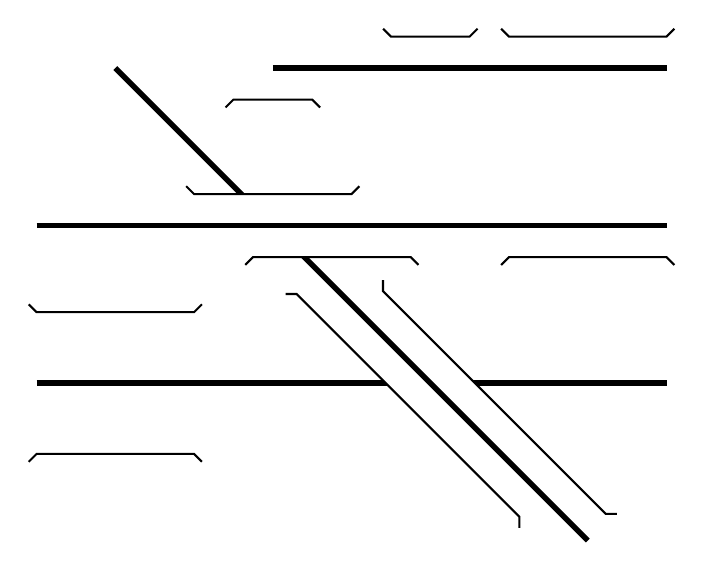
\begin{tikzpicture}
  
    \foreach \i in {1,2,...,4}{% base coordinate
      \coordinate (A\i) at ($(0,0) + 2*(0,-\i)$);% base coordinate
      \coordinate (B\i) at ($(8,0) + 2*(0,-\i)$);% base coordinate
    }


    \foreach \i in {1,2,...,4}{% coordinates for testing symbols
      \coordinate (X\i-1) at ($(1,0) + 2*(0,-\i)$);
      \coordinate (X\i-2) at ($(3,0) + 2*(0,-\i)$);
      \coordinate (X\i-3) at ($(5,0) + 2*(0,-\i)$);
      \coordinate (X\i-4) at ($(7,0) + 2*(0,-\i)$);
    }

    \bridge[length=2cm,width=1cm] at (X3-1);
    \maintrack (A3) -- (B3);
    \bridge[rotate=-45,shift left=0.75cm] at (X3-3);
    \maintrack (X1-1) -- (X4-4);
    \bridge[length=2cm,shift right=0.75cm] at (X2-2);
    \bridge[length=2cm,width=1.5cm] at (7,-3);
    \maintrack (A2) -- (B2);
    \maintrack (X1-2) -- (B1);

    \bridge[no background,length=1cm,side=right] at (X1-2);
    \bridge[no background,length=1cm,side=left]  at (X1-3);

  \end{tikzpicture}
\end{document}